
\section{Under the Hood}
\label{sec:hood}
Now that we have understood our box it is time to start knowing what is inside it. The neural network is composed by several layers. At least we have the input layer (receive the data from outside) and the output layer (give us the prediction). Between those two could be more hidden layers. Each of them has a certain number of neurons $n_1, n_2, .., n_m$ where $m$ is the number of layers. That means that the input layer has $n_1$ neurons while the output layer has $n_m$ neurons. Each neuron of the first layer is connected with each neuron of the second layer, each neuron of the second layer is connected with each neuron of the third layer and so on (See Figure ~\ref{fig:net2}). \\

\begin{figure}
  \center
  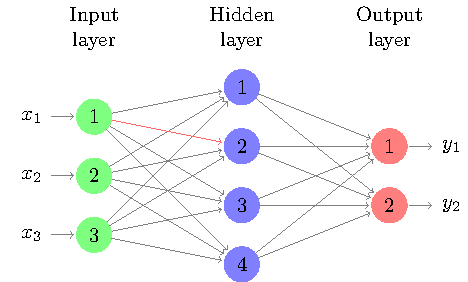
\includegraphics[scale=1.5]{images/net2.pdf}
  \caption{\label{fig:net2}Example of Neural Network with 3 layers. Here $n_1=3$, $n_2=4$ and $n_3=2$. The connection in red is denoted as $w^{(1)}_{12}$ (according to Equation ~\ref{eq:w})}
\end{figure}

Each of those connections has a weight $w$. To denote these weights we are going to use the form $w_{ij}^{(k)}$ where $k$ means which layer the connection departs from, $i$ means which neuron of layer $k$ the connection departs from and $j$ means which neuron of layer $k+1$ the connections arrives to (See Figure ~\ref{fig:net2}). Therefore $w$ is:
\begin{equation}
\begin{aligned}
  & w^{(k)}_{ij} \\
  & i=1,\dots,n_k \\
  & j=1,\dots,n_{k+1} \\
  & k=1,\dots,m
\end{aligned}
\label{eq:w}
\end{equation}\\

Each neuron has a bias that allow set how excited is a neuron. A really excited neuron always output '1' while a non-excited neuron always give us '0'. The bias helps the network to adjust some neurons as important since not every neuron output is equally interesting. The work of a single neuron is as simple as add the bias and the weighted inputs and apply a function to the result ~\cite[Chapter~27]{springer}. The output $o$ of a neuron is:
\begin{equation}
  o^{(k)}_i=
  \begin{cases}
    x_i, & k=1 \\
    f\bigg(u^{(k)}_i+\sum^{n_{k-1}}_{j=1}w^{(k-1)}_{ji}\cdot o^{(k-1)}_j\bigg), & k>1
  \end{cases}
\end{equation}
For example, for the neuron 3 in blue of Figure ~\ref{fig:net2} the output will be $o^{(2)}_3=f(u^{(2)}_3+w^{(1)}_{13}\cdot o^{(1)}_1+w^{(1)}_{23}\cdot o^{(1)}_2+w^{(1)}_{33}\cdot o^{(1)}_3)$. For the same neuron the scheme is showed in Figure ~\ref{fig:neur1}.
\begin{figure}[H]
  \center
  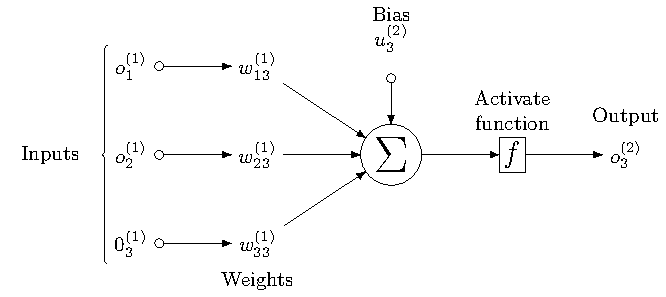
\includegraphics[scale=1]{images/neuron1.pdf}
  \caption{\label{fig:neur1}Example of the task of a single neuron \cite{neurdiag}}
\end{figure}
